

\begin{frame}{Beviser}
    Gitt noen premisser, vis at det garanterer en konklusjon.\\

    Det aller vanskeligste er å finne riktig idé til beviset. Det finnes mange typer bevis, og det er mye rom for kreativitet. Man må bare prøve seg frem.\\
    
    \pause
    Likvel kan vi vanligvis begynne med følgende:
    \begin{enumerate}
        \item Vurder hvorvidt påstanden ser ut til å stemme. Test på noen eksempler, prøv å finne et moteksempel.
        \pause
        \item Skriv opp hva vi vet, og hva vi vil vise, i mattenotasjon.
        \pause
        \item Se etter en sammenheng, grunnen til at det ene impliserer det andre.
        \pause
        \item Gjør resten av beviset.
    \end{enumerate}
\end{frame}

\begin{frame}{Oppgave: vis at om $a$ og $b$ er oddetall, da er $a + b$ et partall.}
    \pause
    \begin{enumerate}
        \item Vi tester med et par eksempler: $3+7 = 10, 15+1 = 16$.
        \pause
        \item Vi vet at $a = 2k + 1$, og $b = 2c + 1$, for noen heltall $k, c$. 
        
        Vi vil vise at $a + b = 2h$, for et heltall $h$.
        \pause
        \item Vi prøver å bare legge dem sammen og se hva som skjer:
        
        $a + b = (2k + 1) + (2c + 1) = 2(k + c + 1)$

        Og da var vi plutselig allerede ferdige.
    \end{enumerate}

    \pause
    \begin{block}{Bevis: summen av to oddetall er et partall}
        La $a = 2k + 1, b = 2c + 1$ være oddetall, for vilkårlige heltall $k$ og $c$.\\\pause
        Da er $a + b = (2k + 1) + (2c + 1) = 2(k + c + 1)$, som er et partall. $\qed$
    \end{block}
\end{frame}

\begin{frame}{Direkte og kontrapositive bevis}
    Et direkte bevis for $p \rightarrow q$ er et som antar at $p$ = T, og viser at det medfører at $q$ = T.
    Dette er ofte de enkleste bevisene. Hvis du har formler du bare må knytte sammen, forsøk det først.\\

    \pause
    Vi gjorde nettopp et direkte bevis: $p =$ "$a$ og $b$ er oddetall", $q =$ "$a+b$ er et partall", og vi viste at $p \rightarrow q$.\\

    \pause
    Siden $p \rightarrow q \equiv \lnot q \rightarrow \lnot p$, kan vi også bevise det 'baklengs': om konklusjon er usann, må premisset også være usannt.
\end{frame}

\begin{frame}{Oppgave: vis at for alle $n$, om $n^2$ er et partall, er $n$ et partall.}
    \begin{enumerate}
        \pause
        \item Vi tester: 64 og 8 er partall, 36 og 6 er partall. Ser riktig ut.
        \pause
        \item Vi vet at $n^2 = 2k$, og vil vise at da er $n = 2c$.
        \pause
        \item Om $n^2$ er et partall, må det antageligvis være et partall ganget med seg selv, ellers får vi et oddetall. Det høres meningsfullt ut, men er kanskje vanskelig å vise rett frem.
    \end{enumerate}

    \pause
    \begin{block}{For alle $n$, om $n^2$ er et partall, er $n$ et partall}
        La $n = 2c + 1$ være et oddetall, for et heltall $c$.

        \pause
        Da er $n^2 = (2c + 1)^2 = 4c^2 + 4c + 1 = 2(2c^2 + 2c) + 1$, som er et oddetall.

        \pause
        Om $n$ er et oddetall er $n^2$ dermed også det. Om $n^2$ er et partall, er $n$ dermed nødt til å være et partall. $\qed$
    \end{block}
\end{frame}

\begin{frame}{Motbevis}
    For å motbevise en påstand, holder det å bare finne et moteksempel. Dette er vanligvis den letteste typen bevis. Det er kun her det er greit å stoppe etter kun et eksempel.
    \pause
    \begin{block}{Påstand: det er ikke mulig å plassere 8 dronninger på et sjakkbrett uten at noen av dem truer hverandre.}
    \pause
    \begin{figure}
        \centering
        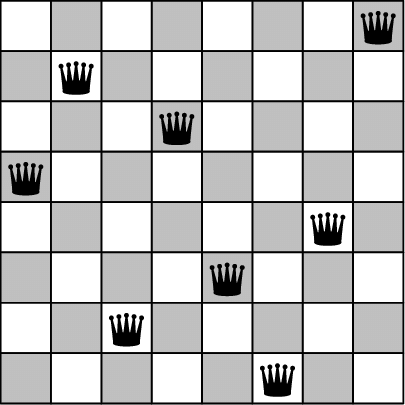
\includegraphics[scale=0.20]{images/8 queens.png}
        \label{fig:my_label}
    \end{figure}
    \end{block}
\end{frame}

\begin{frame}{Motsigelsesbevis (Proof by contradiction)}
    For å bevise en proposisjon $p$, kan vi heller bevise at $\lnot p$ leder til en selvmotsigelse. 
    Vi motbeviser det motsatte.\\

    \pause
    Et motsigelsesbevis ser vanligvis slik ut:
    \begin{block}{Oppgave: vis at $p$ er sant}
        \pause
        Ok da, la oss anta at $p$ på en eller annen måte \emph{ikke} er sant.

        \pause
        Hadde ikke det vært ganske dumt?

        \pause
        Ja nettopp, jeg regner med du føler deg dum nå.

        \pause
        Derfor er $p$ sant.
    \end{block}
\end{frame}

\begin{frame}{Eksempel på et motsigelsesbevis}
    \begin{block}{Summen av et rasjonalt tall $\frac{a}{b}$ og et irrasjonalt tall $c$ også er et irrasjonalt tall.}
        \pause
        Vi antar det motsatte, at summen blir et rasjonalt tall: \\
        \pause
        $\frac{a}{b}$ + $c$ = $\frac{e}{d}$ for $e, d \in \mathbb{Z}$.\\
        \pause
        $\implies \frac{e}{d} - \frac{a}{b} = c$\\
        \pause
        $\implies \frac{b\cdot e - a \cdot d}{b\cdot d} = c$\\[1.5mm]
        \pause
        Men det impliserer jo at $c$ er et rasjonalt tall. \text{\Lightning}\\
        \pause
        Derfor er det usant at summen er et rasjonalt tall.\\
        $\implies$ summen må være irrasjonal.
        \qed
    \end{block}
\end{frame}

\begin{frame}{Uttømmende bevis (Proof by exhaustion)}
    Noen ganger greier vi ikke finne på et elegant bevis. Da tar vi heller for oss hvert enkelt tilfelle hver for seg, og når vi har vist at det holder for absolutt alle tilfeller har vi bevist påstanden. Merk at da må det være et endelig antall tilfeller.
    \pause
    \begin{block}{Vis at alle sommer-OL har blitt arrangert i årstall delelige på 4.}
        \pause
        1896 mod 4 = 0 \checkmark \\
        \pause
        1900 mod 4 = 0 \checkmark \\
        \pause
        {[... de neste 30 linjene er trivielle og etterlatt som en oppgave for leseren ...]}\\
        2024 mod 4 = 0 \checkmark
    \end{block}
    \pause
    Dette er altså ikke et komplett bevis. Vi må faktisk vise alle tilfeller før vi er ferdig.
\end{frame}
